\documentclass[a4paper,12pt]{article}
\usepackage[a4paper,top=1.3cm,bottom=2cm,left=1.5cm,right=1.5cm,marginparwidth=0.75cm]{geometry}
\usepackage{cmap}
\usepackage{mathtext}
\usepackage[T2A]{fontenc}
\usepackage[utf8]{inputenc}
\usepackage[english,russian]{babel}
\usepackage{siunitx}
\usepackage{enumitem}
\usepackage{placeins}

\usepackage{graphicx}

\usepackage{wrapfig}
\usepackage{tabularx}
\usepackage{multirow}

\usepackage{hyperref}
\usepackage[rgb]{xcolor}
\hypersetup{colorlinks=true,urlcolor=blue}
\usepackage{siunitx}
\usepackage{amsmath,amsfonts,amssymb,amsthm,mathtools}
\usepackage{icomma}
\mathtoolsset{showonlyrefs=false}
\usepackage{euscript}
\usepackage{mathrsfs}
\DeclareMathOperator{\sgn}{\mathop{sgn}}
\newcommand*{\hm}[1]{#1\nobreak\discretionary{}
{\hbox{$\mathsurround=0pt #1$}}{}}

%%% Заголовок
\newcommand\labname{Измерение коэффициента ослабления потока $\gamma$-лучей в веществе и определение их энергии}
\newcommand\labnumber{5.1}


\author{Макаров Лев Евгеньевич}
\title{Лабораторная работа №\labnumber

\labname
}

\date{\today}

\begin{document}

\begin{titlepage}
	\begin{center}
		{\large МОСКОВСКИЙ ФИЗИКО-ТЕХНИЧЕСКИЙ ИНСТИТУТ (НАЦИОНАЛЬНЫЙ ИССЛЕДОВАТЕЛЬСКИЙ УНИВЕРСИТЕТ)}
	\end{center}
	\begin{center}
		{\large Физтех-школа фотоники, электроники и молекулярной физики}
	\end{center}
	
	
	\vspace{4.5cm}
	{\huge
		\begin{center}
			{\bf Отчёт о выполнении лабораторной работы \labnumber}\\
			\labname
		\end{center}
	}
	\vspace{2cm}
	\begin{flushright}
		{\LARGE Автор:\\ Макаров Лев Евгеньевич \\
			\vspace{0.2cm}
			Б04-306}
	\end{flushright}
	\vspace{8cm}
	\begin{center}
		Долгопрудный 2025
	\end{center}
\end{titlepage}

\section{Введение}

\textbf{Цель работы:} 
\begin{enumerate}
	\item С помощью сцинтилляционного счетчика измерить линейные коэффициенты ослабления потока $\gamma$-лучей в свинце, железе и алюминии;
    \item По их величине поределить энергию $\gamma$-квантов.
\end{enumerate}

\textbf{В работе используются:} 


\section{Теоретические сведения}

Проходя через вещество, пучок $\gamma$-квантов постепенно ослабляется. Ослабление происходит по экспоненциальному закону, который может быть записан в двух эквивалентных формах:

\begin{equation}\label{eq:1}
    I = I_0 e^{- \mu l}
\end{equation}

\begin{equation}\label{eq:2}
    I = I_0 e^{- \mu' m_1}
\end{equation}

где $I$, $I_0$ — интенсивности прошедшего и падающего излучений, $l$ — длина пути, пройденного пучком $\gamma$-лучей, $m_1$ — масса пройденного вещества, приходящаяся на единицу площади, $\mu$ и $\mu'$ — константы, величина которых зависит от вещества, сквозь которое проходят $\gamma$-лучи.

Ослабление потока $\gamma$-лучей, происходящее при прохождении среды, связано с тремя эффектами: фотоэлектрическим поглощением, комптоновским рассеянием и с генерацией электрон-позитронных пар. Рассмотрим эти эффекты.

\subsection*{Фотоэлектрическое поглощение}

При столкновении $\gamma$-квантов с электронами внутренних атомных оболочек может происходить поглощение квантов. Энергия $\gamma$-кванта передается соответствующему электрону, а импульс делится между этим электроном и оставшимся после его вылета ионом.

Вероятность $dP_\text{Ф}$ фотоэлектрического поглощения $\gamma$-квантов пропорциональна длине пути $dl$ и плотности электронов в среде (в расчет должны приниматься только электроны, принадлежащие внутренним оболочкам атомов):

\begin{equation}\label{eq:3}
    dP_\text{Ф} = \sigma_\text{Ф} n_1 dl
\end{equation}
где $n1$ — плотность внутренних электронов, а $\sigma_\text{Ф}$ — поперечное сечение фотоэлектрического поглощения. Поперечное сечение характеризует вероятность фотоэффекта, рассчитанную на один электрон.

Связь между коэффициентом поглощения $\mu_\text{Ф}$ и сечением $\sigma_\text{Ф}$:

\begin{equation}\label{eq:4}
    \mu_\text{Ф} = \sigma_\text{Ф}n_1
\end{equation}

Формула \eqref{eq:4} выражает зависимость $\mu_\text{Ф}$ от плотности электронов и, следовательно, от плотности среды в явном виде.

Пусть в результате фотоэффекта энергия $\gamma$-кванта передается электрону, находящемуся на $i$-й оболочке атома. Обозначим через $W_i$ энергию связи этого электрона. После вылета из атома электрон приобретает кинетическую энергию

\begin{equation}\label{eq:5}
    T_i = \hbar w - W_i
\end{equation}

Освободившееся после вылета электрона место заполняется затем одним из электронов с вышележащих оболочек. При таких переходах возникает характеристическое рентгеновское излучение*).

Вероятность фотоэффекта сложным образом зависит от энергии $\gamma$-лучей и от заряда ядер. Для оценок можно пользоваться формулой

\begin{equation}\label{eq:6}
    \sigma_\text{Ф} \propto \frac{Z^5}{\left( \hbar w \right)^{3,5}}
\end{equation}

правильно передающей основные черты явления. Из формулы \eqref{eq:6} видно, что вероятность фотоэффекта быстро возрастает при переходе от легких к тяжелым элементам и резко падает с увеличением энергии $\gamma$-квантов.


\begin{figure}[h]
    \begin{center}
        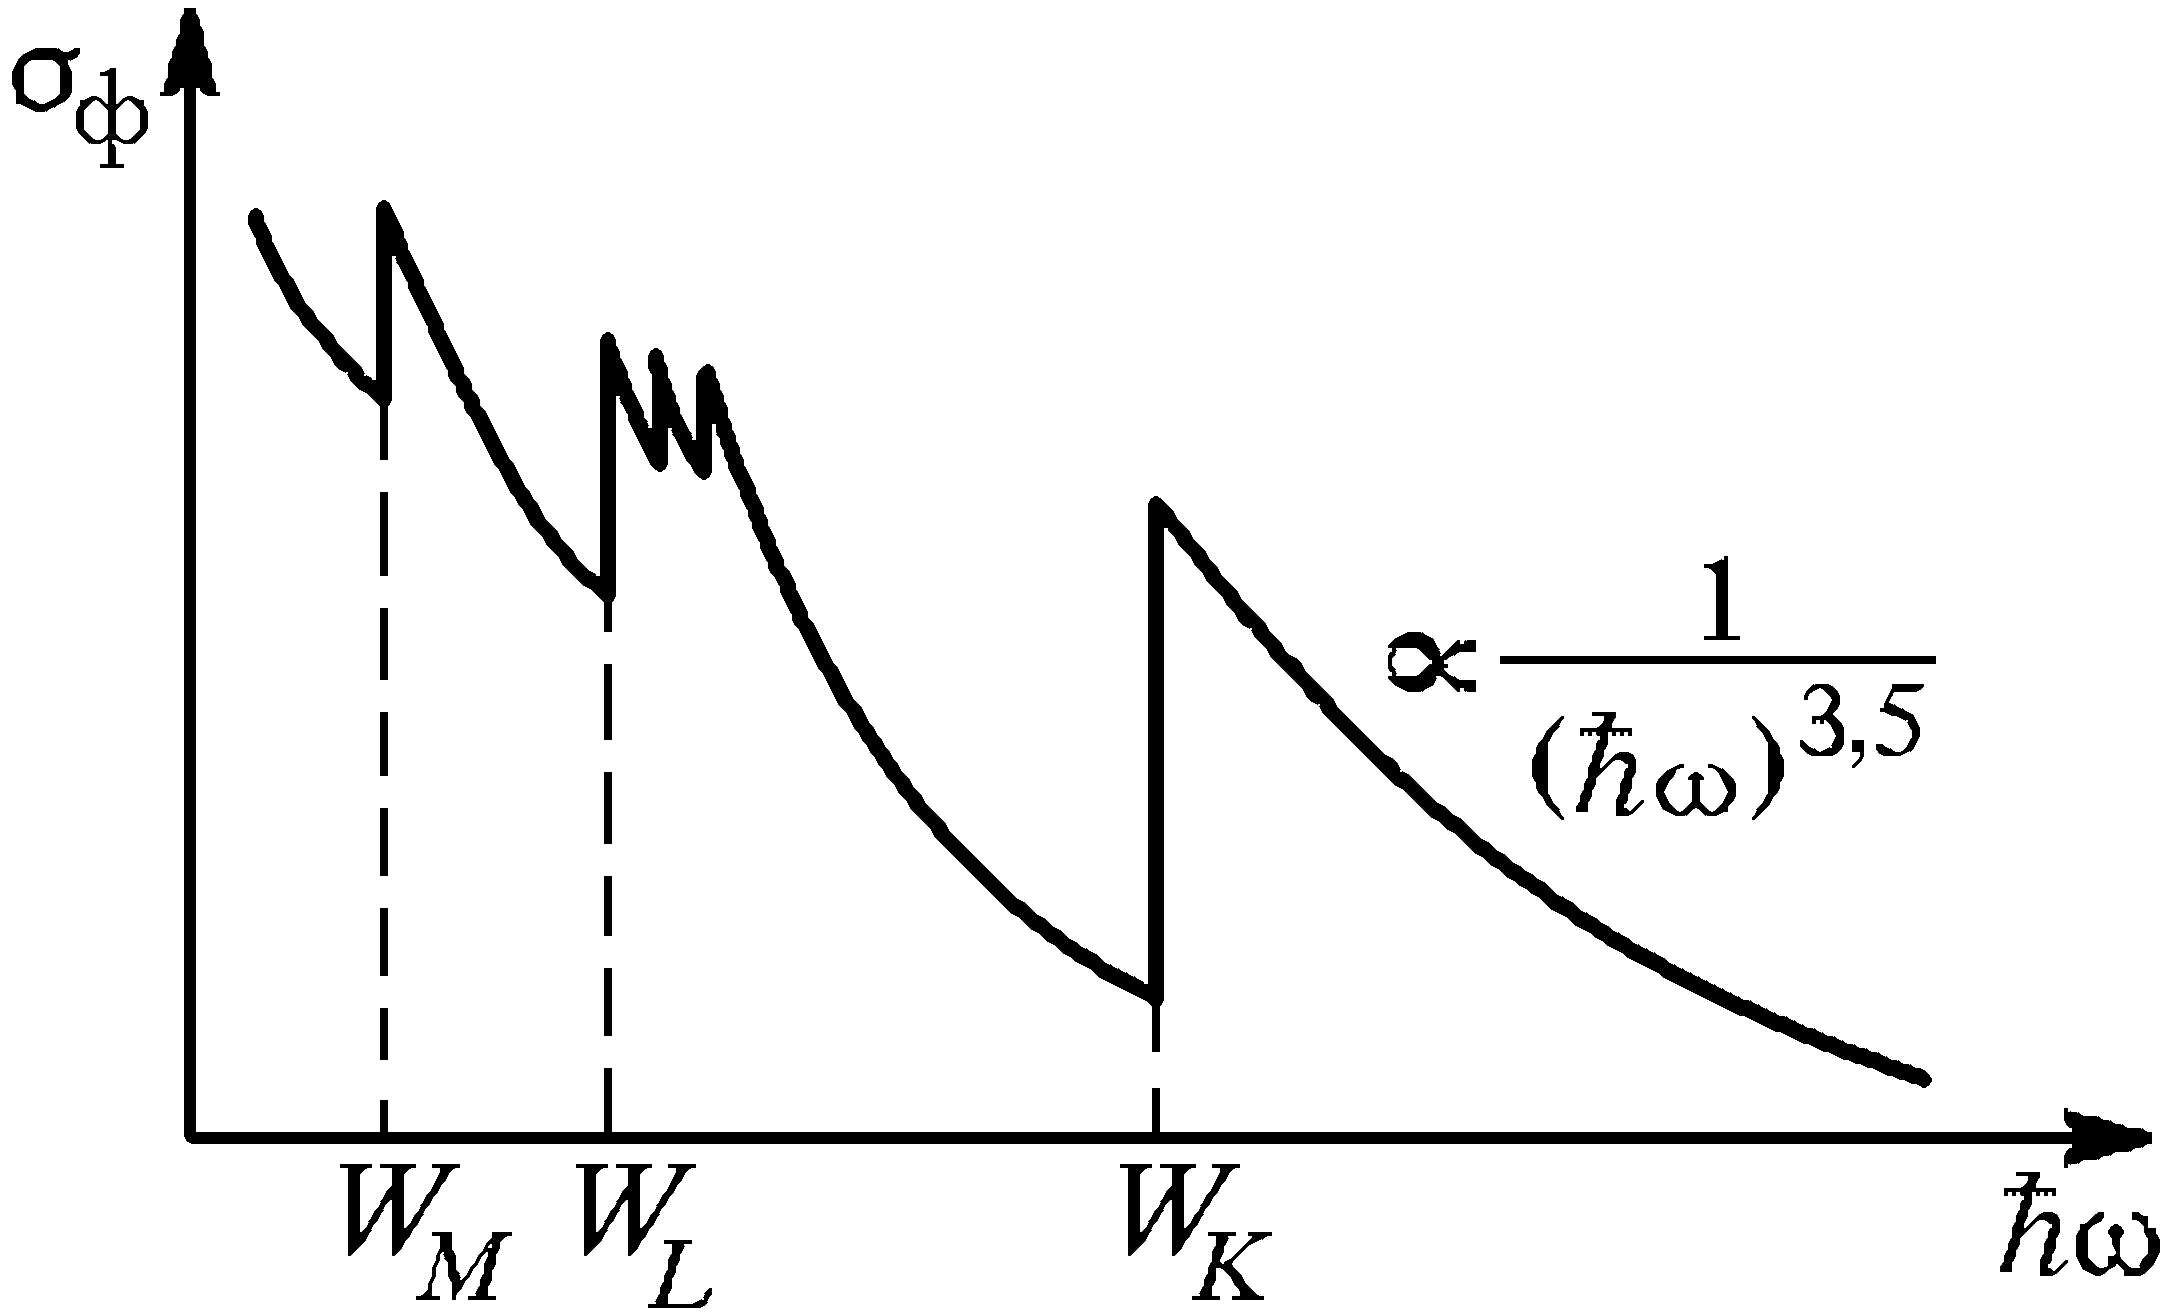
\includegraphics[width = 0.5\textwidth]{pictures/area_energy.png}
        \caption{Зависимость сечения фотоэффекта от энергии $\gamma$-квантов}
    \label{pic:area_energy}
    \end{center}
\end{figure}


На рис. \ref{pic:area_energy} показана энергетическая зависимость сечения фотоэффекта. Из рисунка видно, что при энергиях $\gamma$-квантов, лежащих в области атомных энергий связи, сечение претерпевает резкие изменения: при возрастании энергии это сечение скачкообразно возрастает, когда становится возможным выбивание электронов с очередной оболочки (на рис. \ref{pic:area_energy} это скачки при энергиях $W_M$, $W_L$, $W_K$, соответствующих энергиям связи $M$ , $L$ и $K$-электронов). В этой области сечение фотоэффекта очень велико по сравнению с сечениями других процессов. Поэтому фотоэффект является доминирующим механизмом поглощения $\gamma$-квантов при не очень высоких энергиях.

\subsection*{Комптоновское рассеяние}

Комптоновским рассеянием (или комптон-эффектом) называется упругое столкновение $\gamma$-кванта с электроном. При таком столкновении $\gamma$-квант передает электрону часть своей энергии, величина которой определяется углом рассеяния.

Вероятность комптон-эффекта сложным образом зависит от энергии $\gamma$-квантов. В том случае, когда энергия $\gamma$-кванта много больше энергии покоя электрона, формула сильно упрощается, и выражение для сечения комптон-эффекта приобретает простой вид:

\begin{equation}\label{eq:7}
    \sigma_K = \pi r^2 \frac{mc^2}{\hbar w} \left( \ln {\frac{2 \hbar w}{mc^2}} + \frac{1}{2} \right)
\end{equation}

где $r \simeq 2{,}8 \cdot 10^{-13}$ см — классический радиус электрона, а $m$ — его масса. Из формулы \eqref{eq:7} следует, что сечение комптон-эффекта с ростом энергии фотонов падает далеко не так резко, как сечение фотоэффекта. 

Связь между коэффициентом поглощения $\mu_K$ и сечением $\sigma_K$:

\begin{equation*}
    \mu_K = \sigma_Kn
\end{equation*}

где $n$ - плотность слабосвязанных электронов в веществе.

\subsection*{Образование пар}

При энергиях $\gamma$-лучей, превышающих $2mc^2 = 1{,}02 \ \text{МэВ}$, становится возможен процесс поглощения $\gamma$-лучей, связанный с образованием электрон-позитронных пар. Рождение пар не может происходить в вакууме, оно возникает в электрическом поле ядер. Вероятность этого процесса приблизительно пропорциональна $Z^2$ и сложным образом зависит от энергии фотона. При энергиях больше $2mc^2$ фотоэффект даже для самых тяжелых ядер уже не играет практически никакой роли. Вероятность образования пар должна поэтому сравниваться с вероятностью комптоновского рассеяния. При энергиях, с которыми приходится иметь дело при изучении ядер, рождение пар существенно только в самых тяжелых элементах.

\subsection*{Полный коэффициент ослабления потока $\gamma$-лучей}

Полный линейный коэффициент $\mu$ ослабления пучка $\gamma$-квантов при прохождении через вещество равен сумме коэффициентов для всех трех рассмотренных процессов.

На рис. \ref{pic:mu_for_materials} изображены графики $\mu$ для различных материалов.

\begin{figure}[h]
    \begin{center}
        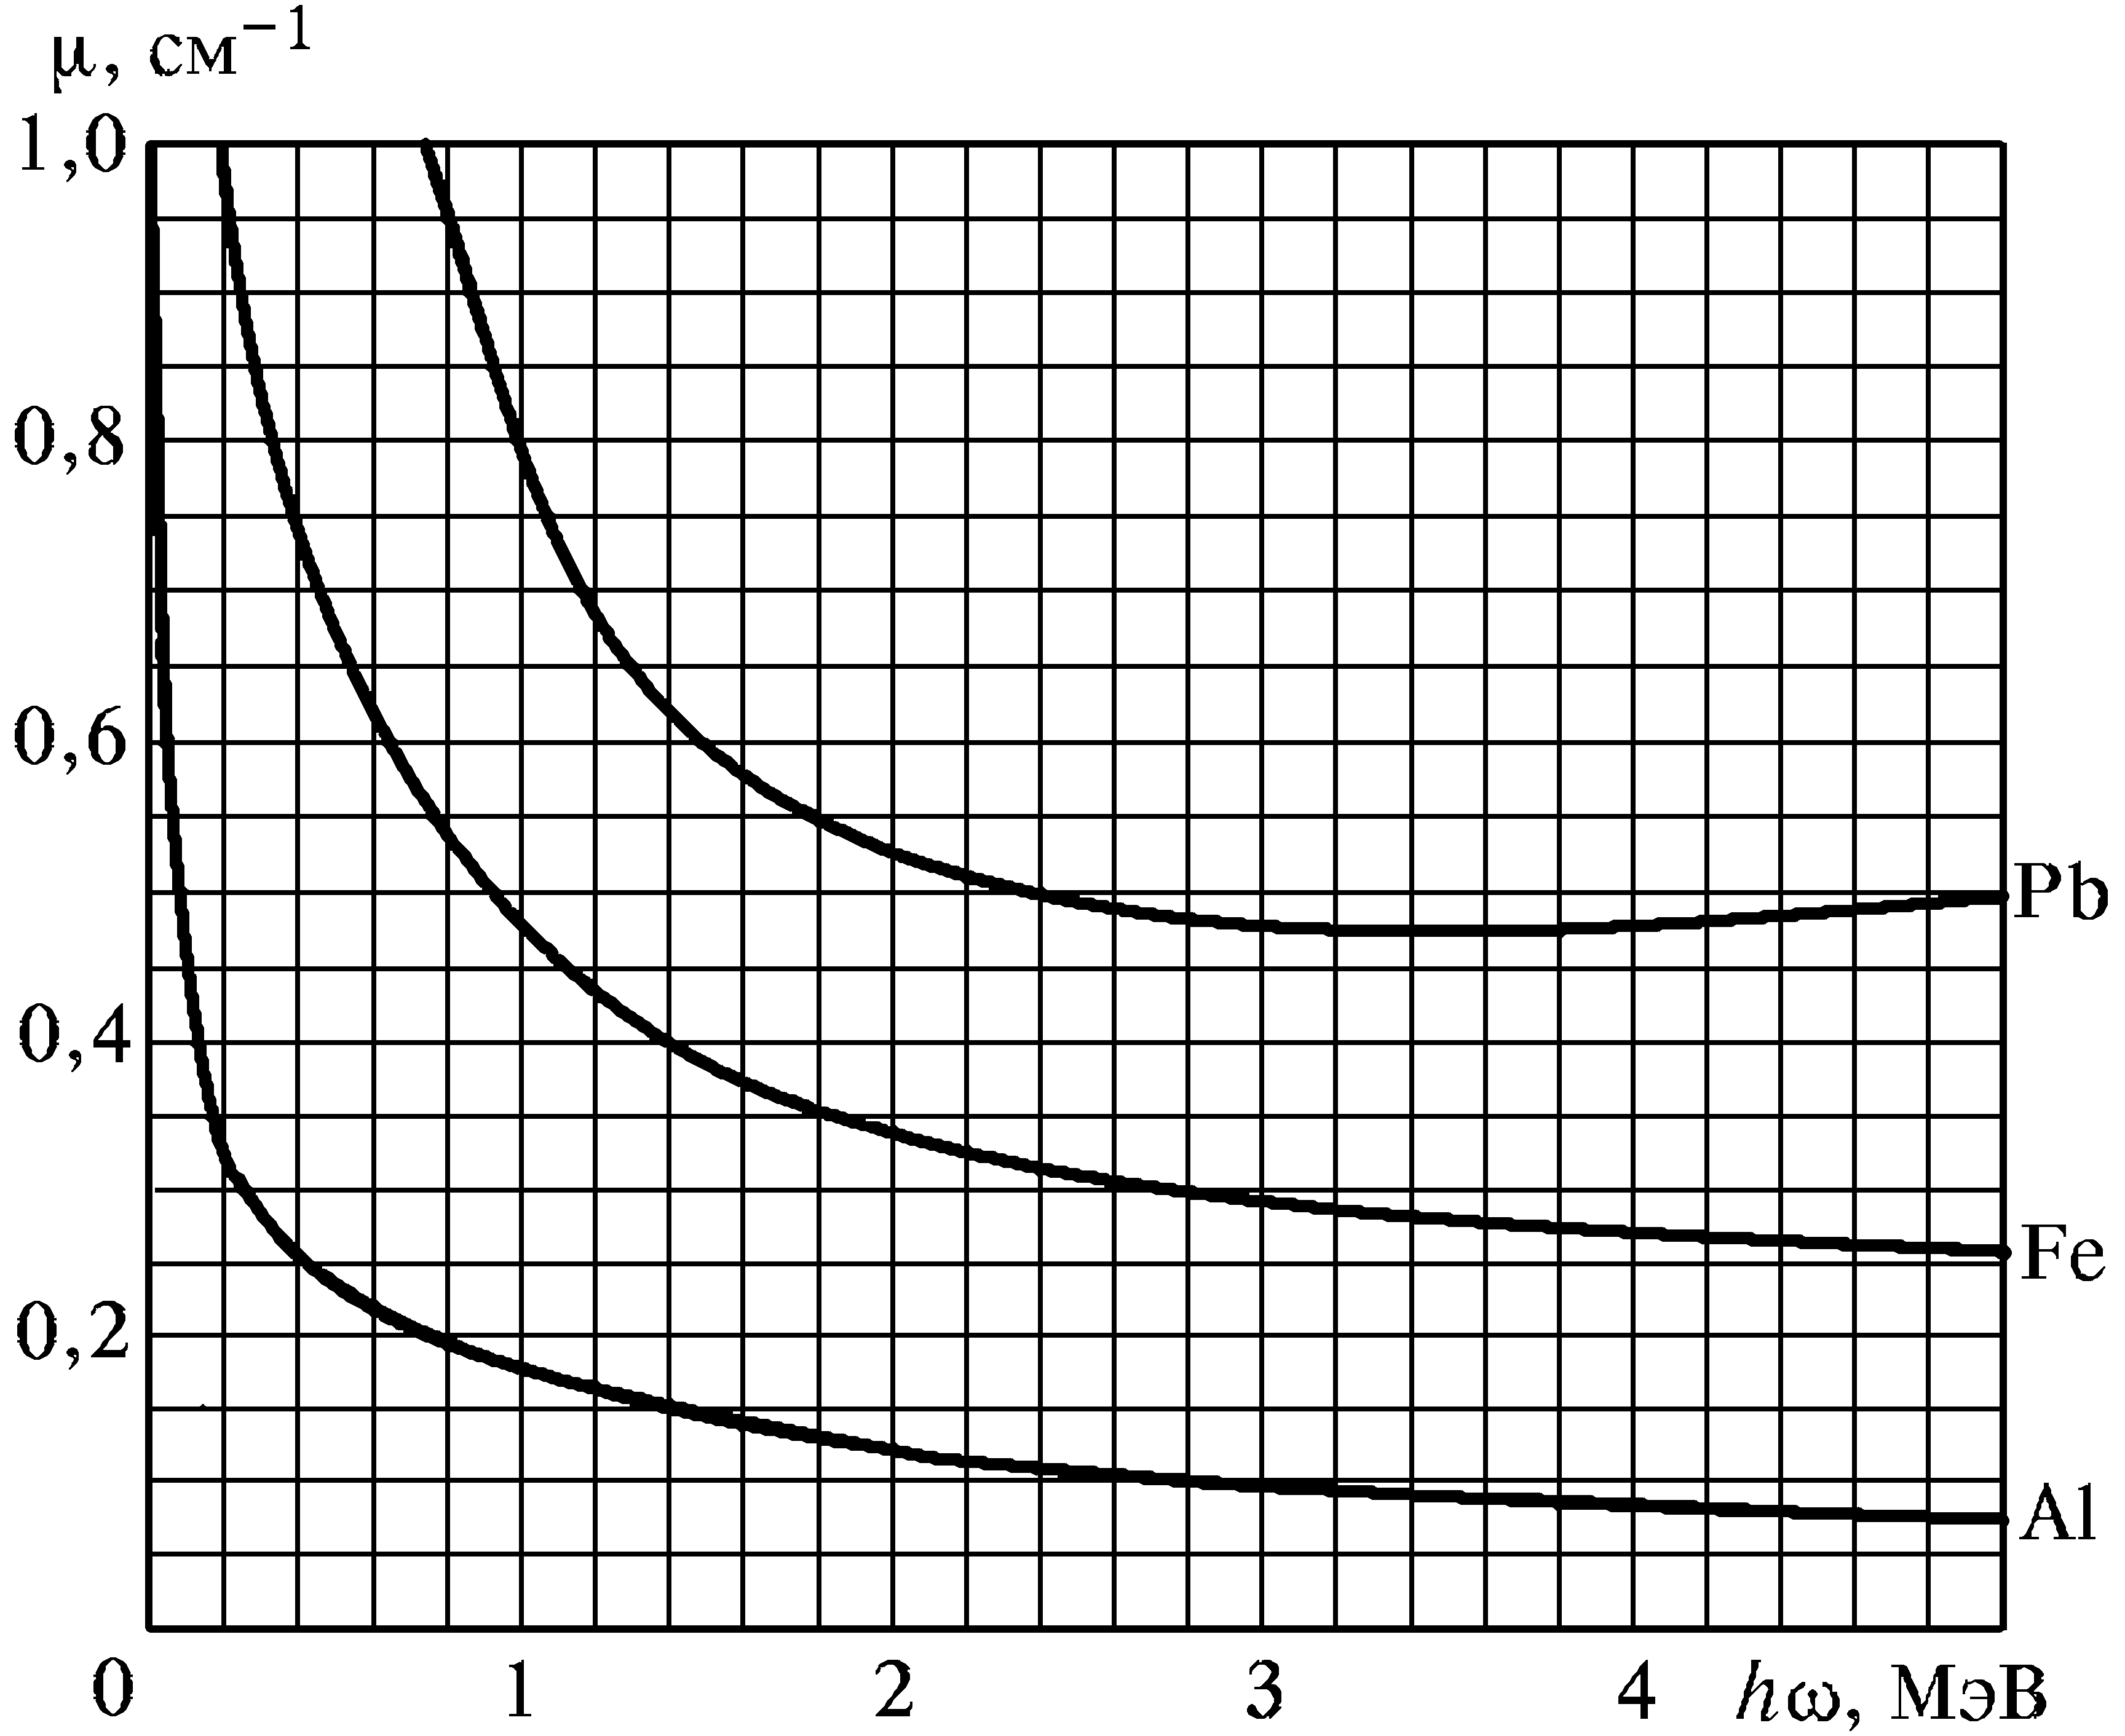
\includegraphics[width = 0.65\textwidth]{pictures/mu_for_Al_Fe_Pb.png}
        \caption{Полные коэффициенты ослабления потока $\gamma$-лучей в алюминии, железе и свинце}
    \label{pic:mu_for_materials}
    \end{center}
\end{figure}

Формулу \eqref{eq:1} нетрудно получить из теоретических соображений. Рассмотрим опыты, поставленные в хорошей геометрии, т. е. в условиях, когда исследуется прохождение сквозь вещество узкого параллельного пучка $\gamma$-лучей. В этом случае не только фотоэлектрическое поглощение и генерация пар, но и комптоновское рассеяние выводит $\gamma$-кванты из пучка.

Поэтому при прохождении через вещество меняется только количество, но не энергия $\gamma$-квантов в пучке, так что коэффициент $\mu$, характеризующий поглощение $\gamma$-квантов в веществе, не зависит от длины пути. Обозначим через $-dN$ число $\gamma$-квантов, выбывших из пучка на пути $dl$. Это число пропорционально имеющемуся их числу $N$ и пройденному пути $dl$. Имеем, следовательно,

\begin{equation}\label{eq:8}
    -dN = \mu N  dl
\end{equation}

Интегрируя уравнение от нулевой длины до заданной, получим \eqref{eq:1}.


В данной работе коэффициент ослабления $\mu$ измеряется в хорошей геометрии. Из формулы \eqref{eq:1} имеем

\begin{equation}\label{eq:9}
    \mu = \frac{1}{l} \ln{\frac{N_0}{N}}
\end{equation}

Для определения коэффициента ослабления нужно, таким образом, измерить толщину образца $l$, число падающих частиц $N_0$ и число частиц $N$ , прошедших через образец.

\section{Экспериментальная установка}

Схема установки представлена на рис. \ref{pic:ustan}

\begin{figure}[h]
    \begin{center}
        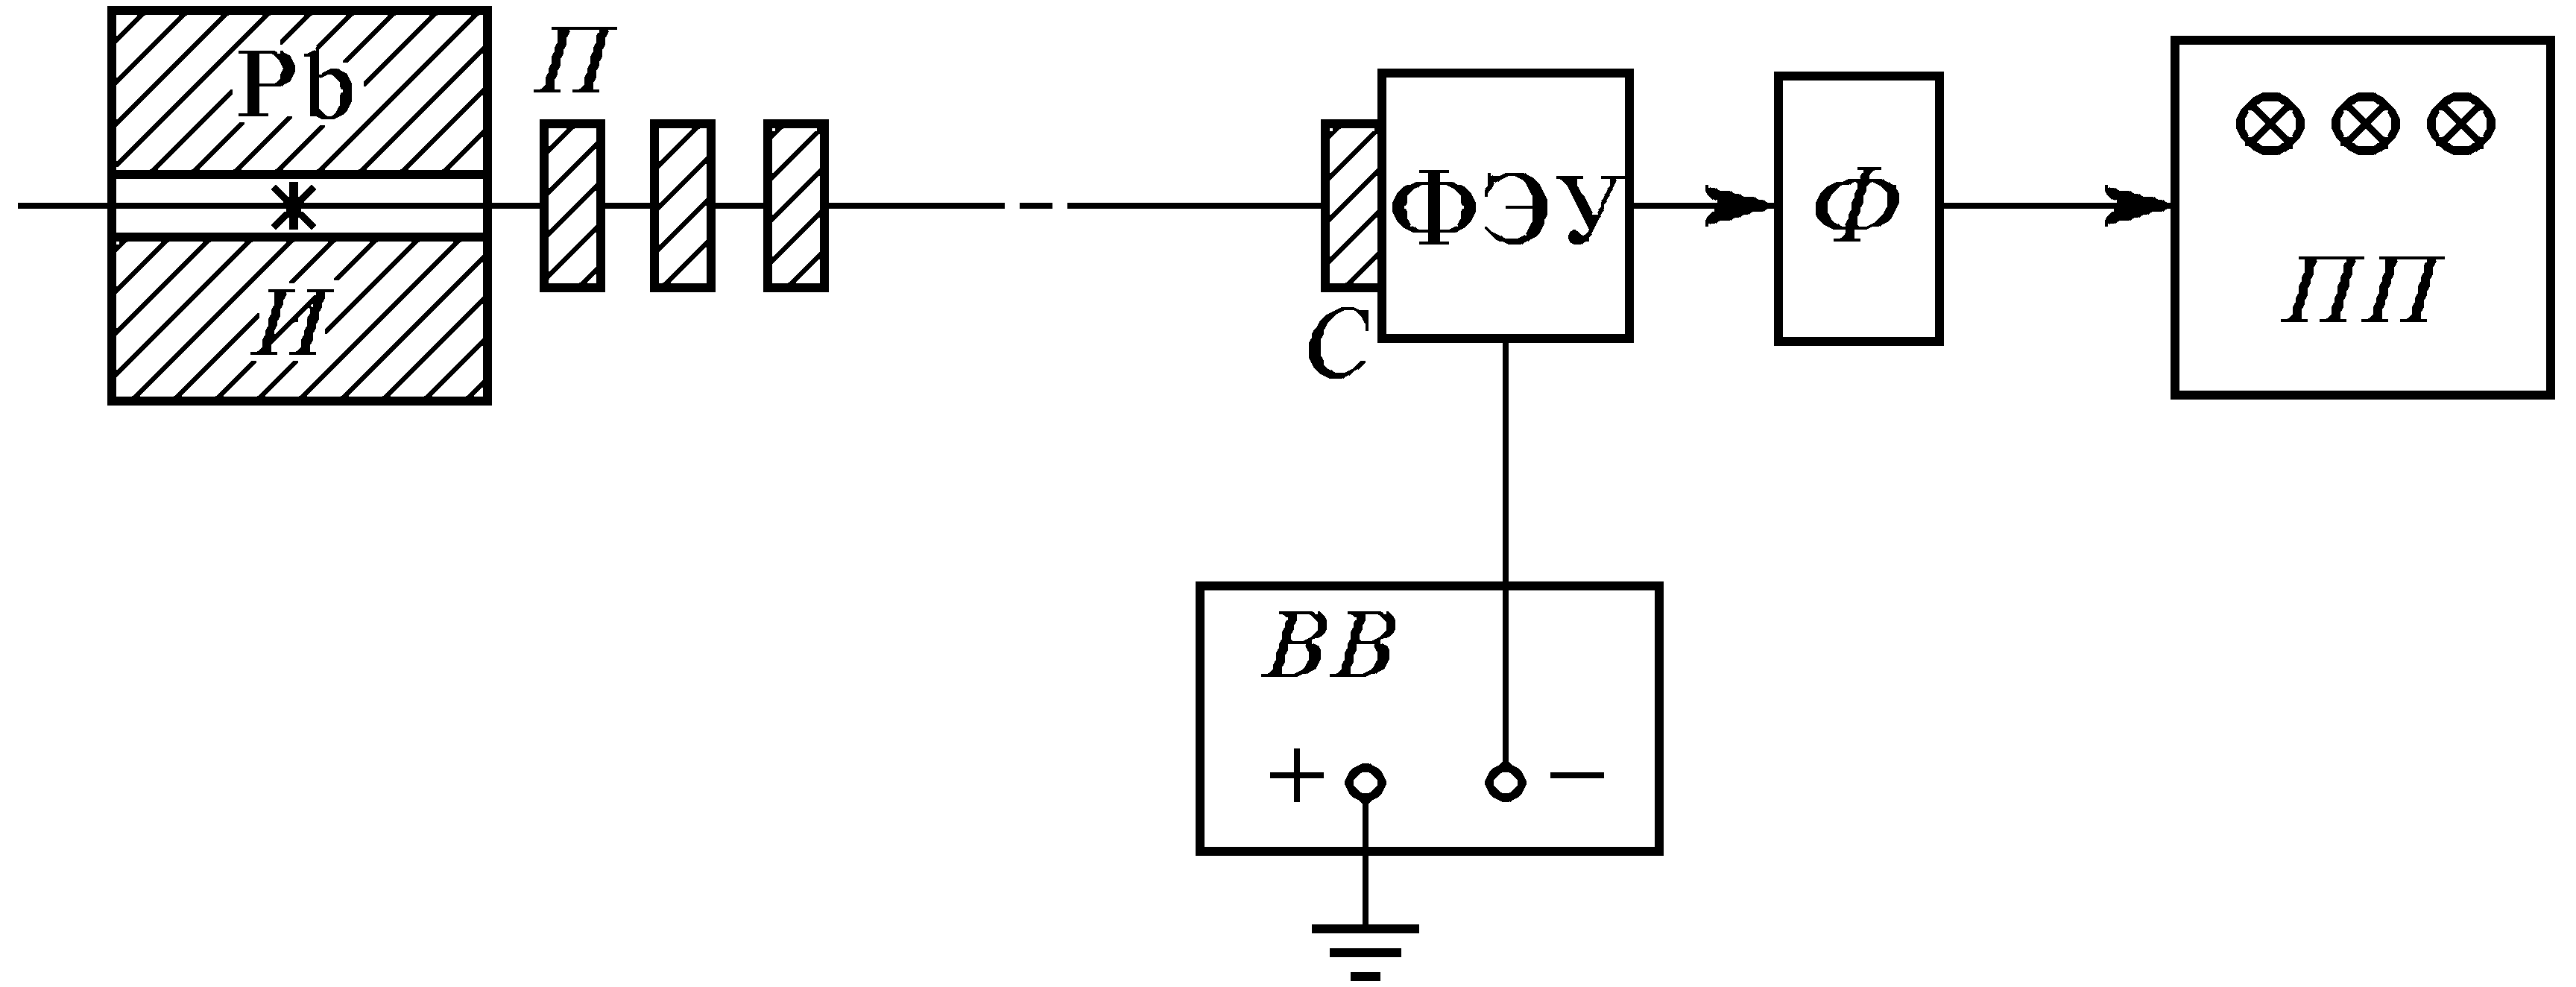
\includegraphics[width = 0.65\textwidth]{pictures/ustan.png}
        \caption{Блок-схема установки, используемой для измерения коэффициентов ослабления потока $\gamma$-лучей: И — источник $\gamma$-лучей; Pb — свинцовый контейнер с коллиматорным каналом; П — набор поглотителей; С — сцинтиллятор — кристалл NaI(Tl); Ф — формирователь-выпрямитель}
    \label{pic:ustan}
    \end{center}
\end{figure}

Свинцовый коллиматор выделяет узкий почти параллельный пучок $\gamma$-квантов, проходящий через набор поглотителей П и регистрируемый сцинтилляционным счетчиком*. Сигналы от счетчика усиливаются и регистрируются пересчетным прибором ПП. Высоковольтный выпрямитель ВВ обеспечивает питание сцинтилляционного счетчика.

При недостаточно хорошей геометрии в результаты опытов могут вкрасться существенные погрешности. В реальных установках всегда имеется конечная вероятность того, что $\gamma$-квант провзаимодействует в поглотителе несколько раз до того, как попадет в детектор (пути таких квантов показаны на рис. \ref{pic:distortion}).


\begin{figure}[h]
    \begin{center}
        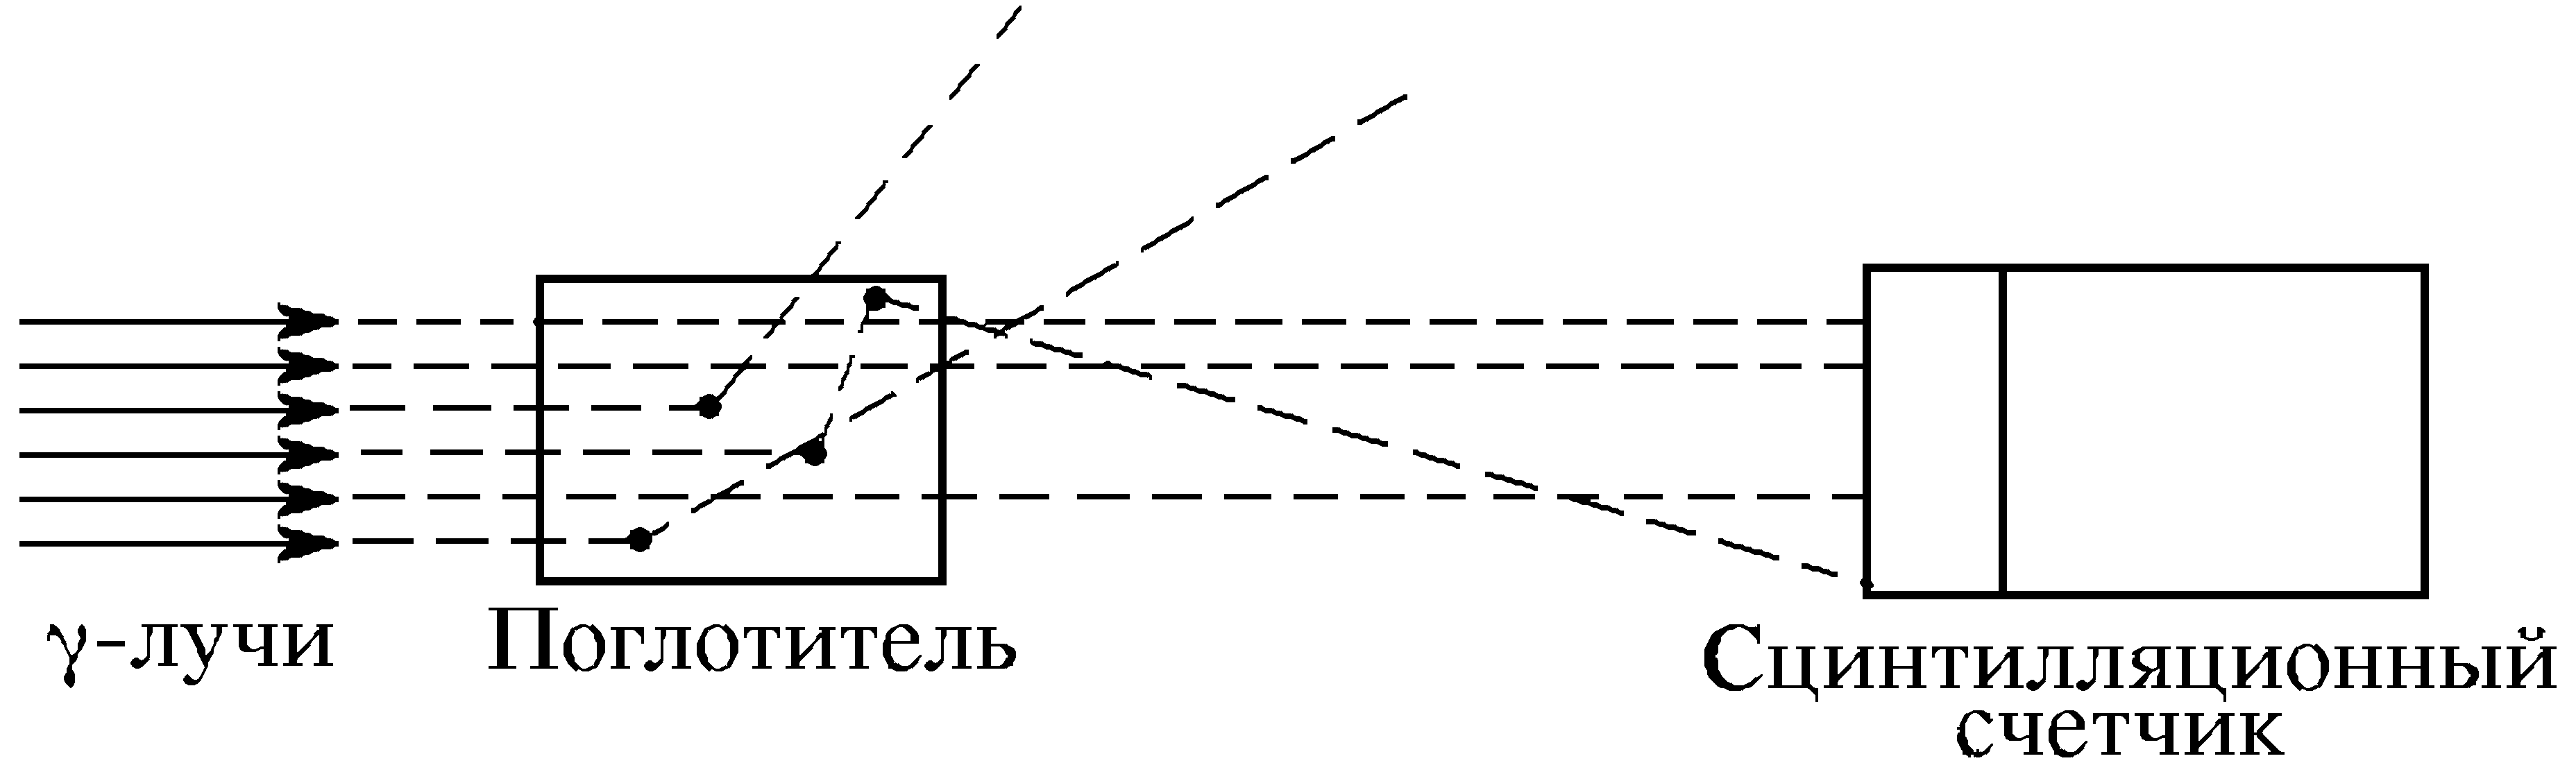
\includegraphics[width = 0.65\textwidth]{pictures/distortion.png}
        \caption{Схема рассеяния $\gamma$-квантов в поглотителе}
    \label{pic:distortion}
    \end{center}
\end{figure}

Чтобы уменьшить число таких случаев, сцинтилляционный счетчик расположен на большом расстоянии от источника $\gamma$-квантов, а поглотители имеют небольшие размеры.

\section{Результаты измерений и обработка данных}

\begin{enumerate}
    \item Включим пересчетный прибор и высоковольтный выпрямитель. Дадим им прогреться в течение 5–10 минут.
    \item Убедитесь в том, что установка «чувствует» $\gamma$-лучи.
\end{enumerate}

Подадим на ФЭУ напряжение 1500 В. Измерьте скорость счета при полностью открытом коллиматоре: $14301$ частиц/с, а затем при коллиматоре, закрытом свинцовой пробкой: $56$ частиц/с

Скорость счета должна резко уменьшиться. Чтобы убедиться в работоспособности установки, повторим эту процедуру 3 раза, результаты измерений запишем в таблицу \ref{table:1}.

\FloatBarrier
\begin{table}[!ht]
    \centering
    \begin{tabular}{|l|l|l|l|l|l|}
        \hline
        $№$ & $t$, с  & $N_\text{закр} \cdot t$, ч & $N_\text{закр}$, ч/с & $N_\text{откр} \cdot t$, ч & $N_\text{откр}$, ч/с \\ \hline
        1      & 20 & 1123   & 56            & 286020 & 14301       \\ \hline
        2      & 20 & 1086   & 54            & 287013 & 14351       \\ \hline
        3      & 20 & 726    & 36            & 287875 & 14394       \\ \hline
    \end{tabular}
    \caption{Измерение скорости счета при открытом и закрытом коллиматоре}
    \label{table:1}
\end{table}
\FloatBarrier

Как видно при закрытом коллиматоре скорость меньше на несколько порядков, значит можем считать, что установка работает. На этом этапе погрешности не вычисляем, потому что это качественное наблюдение работоспособности установки.


\begin{enumerate}[resume]
    \item Исследуем поглощение $\gamma$-лучей в свинце, железе и алюминии.
\end{enumerate}

При всех дальнейших измерениях приборную погрешность датчика учитывать не будем, так как она вносит пренебрежимо малый вклад в сравнении со случайной ошибкой. Приборная погрешность встроенного секундомера не превышает 0.05 с, так как он электронный, а измеряемые периоды времени почти все превышают 100 с. \\

Сначала вычислим фон, который обусловлен шумом ФЭУ и посторонними частицами. Закроем коллиматор толстой свинцовой пробкой. Оставшийся счет не связан, очевидно, с квантами, летящими в пучке. Будем вычитать фон из всех измерений. Результаты измерений фона представлены в таблице \ref{table:2}.

\FloatBarrier
\begin{table}[!ht]
    \centering
    \begin{tabular}{|l|l|l|l|l|}
        \hline
        $№$ & $N \cdot t$, ч & $t$, с & $N$, ч/c & $\left(N_i - \overline{N}\right)^2$, $\text{ч}^2/\text{с}^2$ \\ \hline
        1   & 5690  & 150 & 38 & ~ \\ \hline
        2   & 7227  & 150 & 48 & 13.6  \\ \hline
        3   & 7595  & 150 & 51 & 1.5   \\ \hline
        4   & 9060  & 180 & 50 & 2.4   \\ \hline
        5   & 9744  & 180 & 54 & 5.1   \\ \hline
        6   & 10093 & 180 & 56 & 17.7  \\ \hline
    \end{tabular}
    \caption{Измерение фонового шума}
    \label{table:2}
\end{table}
\FloatBarrier

Случайную погрешность вычислим по формуле (точку под номером 1 считаем выбросом и не учитываем): $\sigma^\text{случ}_\text{шум} = \sqrt{\frac{1}{n - 1} \sum\limits_{i} \left(N_i - \overline{N}\right)^2} \approx 3 \ \text{ч}/\text{с}$ \\


Тогда значение фонового шума:

\begin{equation*}
    N_\text{шум} = (52 \pm 3 ) \ \text{ч}/\text{с}
\end{equation*}

Измерим число частиц, попадающих в счетчик за фиксированное время в отсутствие ($N_0$) поглотителя. Результаты измерений представлены в таблице \ref{table:3}.

\FloatBarrier
\begin{table}[!ht]
    \centering
    \begin{tabular}{|l|l|l|l|l|}
        \hline
        $№$ & $N_0' \cdot t$, ч & $t$, с & $N_0'$, ч/c & $\left({N_0'}_i - \overline{N_0'}\right)^2$, $\text{ч}^2/\text{с}^2$ \\ \hline
        1   & 360522  & 25 & 14421 & 30 \\ \hline
        2   & 359744  & 25 & 14390 & 1338  \\ \hline
        3   & 361709  & 25 & 14468 & 1766   \\ \hline
    \end{tabular}
    \caption{Измерение скорости счета при отсутствии образцов без учета фонового шума}
    \label{table:3}
\end{table}
\FloatBarrier

Погрешность вычислена аналогична шуму. Тогда скорость счета без учета шума: $N_0' = (1442 \pm 4) \cdot 10 \ \text{ч}/\text{с}$

Учтем шум: $N_0 = N_0' - N_\text{шум}$, погрешность вычислим как $\sigma_{N_0} = \sqrt{\sigma^2_\text{шум} + \sigma^2_{N_0'}}$

Тогда

\begin{equation*}
    N_0 = (1437 \pm 4) \cdot 10 \ \text{ч}/\text{с}
\end{equation*}

Измерим толщину образцов штангенциркулем. Результаты измерений запишем в таблицу \ref{table:4}. Пробка при выполнении работы не использовалась, поэтому ее не измеряем.

\FloatBarrier
\begin{table}[!ht]
    \centering
    \begin{tabular}{|l|l|l|l|}
        \hline
        ~ & $l_{Al}$, мм & $l_{Fe}$, мм & $l_{Pb}$, мм \\ \hline
        1 & 20.0 & 10.2 & 4.5 \\ \hline
        2 & 20.0 & 10.1 & 4.7 \\ \hline
        3 & 20.0 & 10.4 & 5.2 \\ \hline
        4 & 19.9 & 10.2 & 4.3 \\ \hline
        5 & 20.1 & ~    & 4.9 \\ \hline
        6 &  ~   &    ~ & 4.9 \\ \hline
        <...> & 20.0 & 10.2 & 4.8 \\ \hline
        $\sigma_l$, мм & 0.2 & 0.2 & 0.7 \\ \hline
    \end{tabular}
    \caption{Измерение толщины образцов}
    \label{table:4}
\end{table}
\FloatBarrier

погрешность считалась как: $\sigma_l = \sqrt{\sigma^2_\text{шт} + \sigma^2_\text{случ}}$, где $\sigma_\text{шт} = 0.05$ мм - приборная погрешность штангенциркуля. \\



Измерим поглощение $\gamma$-лучей при различных толщинах образцов. Коэффициент ослабления потока $\gamma$-квантов вычисляется по формуле \eqref{eq:9}. Для каждой толщины проведем несколько измерений и вычислим случайную погрешность, в таблицы \ref{table:5}, \ref{table:6} и \ref{table:7} сразу запишем итоговые значения для каждой толщины.
Так же сразу учтем фоновый шум и погрешность для каждой скорости пересчитаем аналогично погрешности для $N_0$. \\

Так же посчитаем величину $\ln \frac{N_0}{N}$ и оценим величину ее погрешности по формуле: $\sigma_\text{ln} = \sqrt{\left(\frac{\sigma_{N_0}}{N_0}\right)^2 + \left(\frac{\sigma_{N}}{N}\right)^2}$


\FloatBarrier
\begin{table}[!ht]
    \centering
    \begin{tabular}{|l|l|l|l|l|l|l|}
        \hline
          & $l$, см    & $\sigma_l$, см & $N$, ч/с & $\sigma_N$, ч/с & $\ln \frac{N_0}{N}$  & $\sigma_\text{ln}$ \\ \hline
        1 & 2.00 & 0.02     & 5860  & 30    & 0.390 & 0.006      \\ \hline
        2 & 6.00 & 0.05     & 1420  & 10    & 1.006 & 0.008      \\ \hline
        3 & 10.0 & 0.1      & 199   & 3     & 1.86  & 0.02       \\ \hline
    \end{tabular}
    \caption{Измерение коэффициента поглощения для Al}
    \label{table:5}
\end{table}

\begin{table}[!ht]
    \centering
    \begin{tabular}{|l|l|l|l|l|l|l|}
        \hline
          & $l$, см    & $\sigma_l$, см & $N$, ч/с & $\sigma_N$, ч/с & $\ln \frac{N_0}{N}$  & $\sigma_\text{ln}$ \\ \hline
        1 & 1.02 & 0.02     & 7470  & 10    & 0.285 & 0.003      \\ \hline
        2 & 3.1  & 0.1      & 2540  & 10    & 0.753 & 0.005      \\ \hline
        3 & 4.1  & 0.1      & 1458  & 3     & 0.994 & 0.003      \\ \hline
    \end{tabular}
    \caption{Измерение коэффициента поглощения для Fe}
    \label{table:6}
\end{table}

\begin{table}[!ht]
    \centering
    \begin{tabular}{|l|l|l|l|l|l|l|}
        \hline
          & $l$, см    & $\sigma_l$, м & $N$, ч/с & $\sigma_N$, ч/с & $\ln \frac{N_0}{N}$  & $\sigma_\text{ln}$ \\ \hline
        1 & 0.5 & 0.1      & 792  & 2    & 0.259 & 0.004      \\ \hline
        2 & 1.4 & 0.2      & 2837  & 3     & 0.705 & 0.003      \\ \hline
        3 & 2.4 & 0.4      & 966   & 3     & 1.173 & 0.004      \\ \hline
        4 & 2.9 & 0.4      & 591   & 3     & 1.386 & 0.006      \\ \hline
    \end{tabular}
    \caption{Измерение коэффициента поглощения для Pb}
    \label{table:7}
\end{table}
\FloatBarrier



Построим кривые зависимости логарифма числа сосчитанных частиц от толщины образца для всех исследуемых веществ. Укажем на графиках ошибки измерений.


\FloatBarrier
\begin{figure}[!ht]
        \centering
	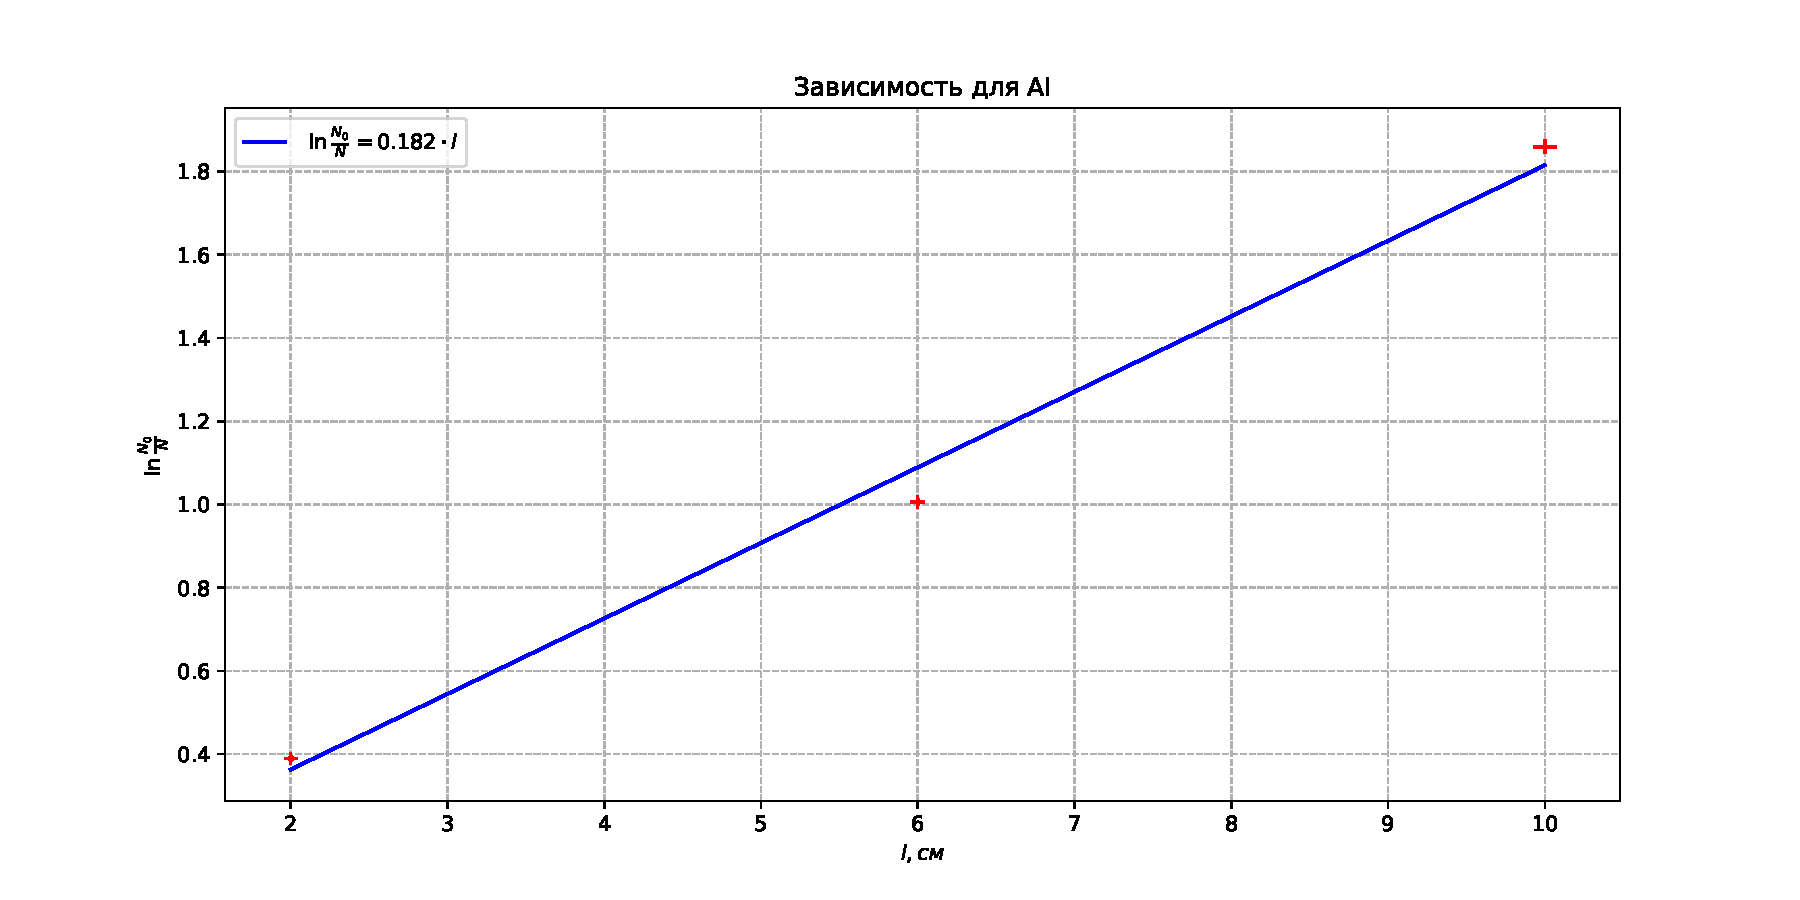
\includegraphics[width=1.0\textwidth]{pictures/graph_Al.pdf}
	\caption{\textit{Зависимость $\ln \frac{N_0}{N}$ от $l$ для Al}}
	\label{graph:1}
\end{figure}

\begin{figure}[!ht]
        \centering
	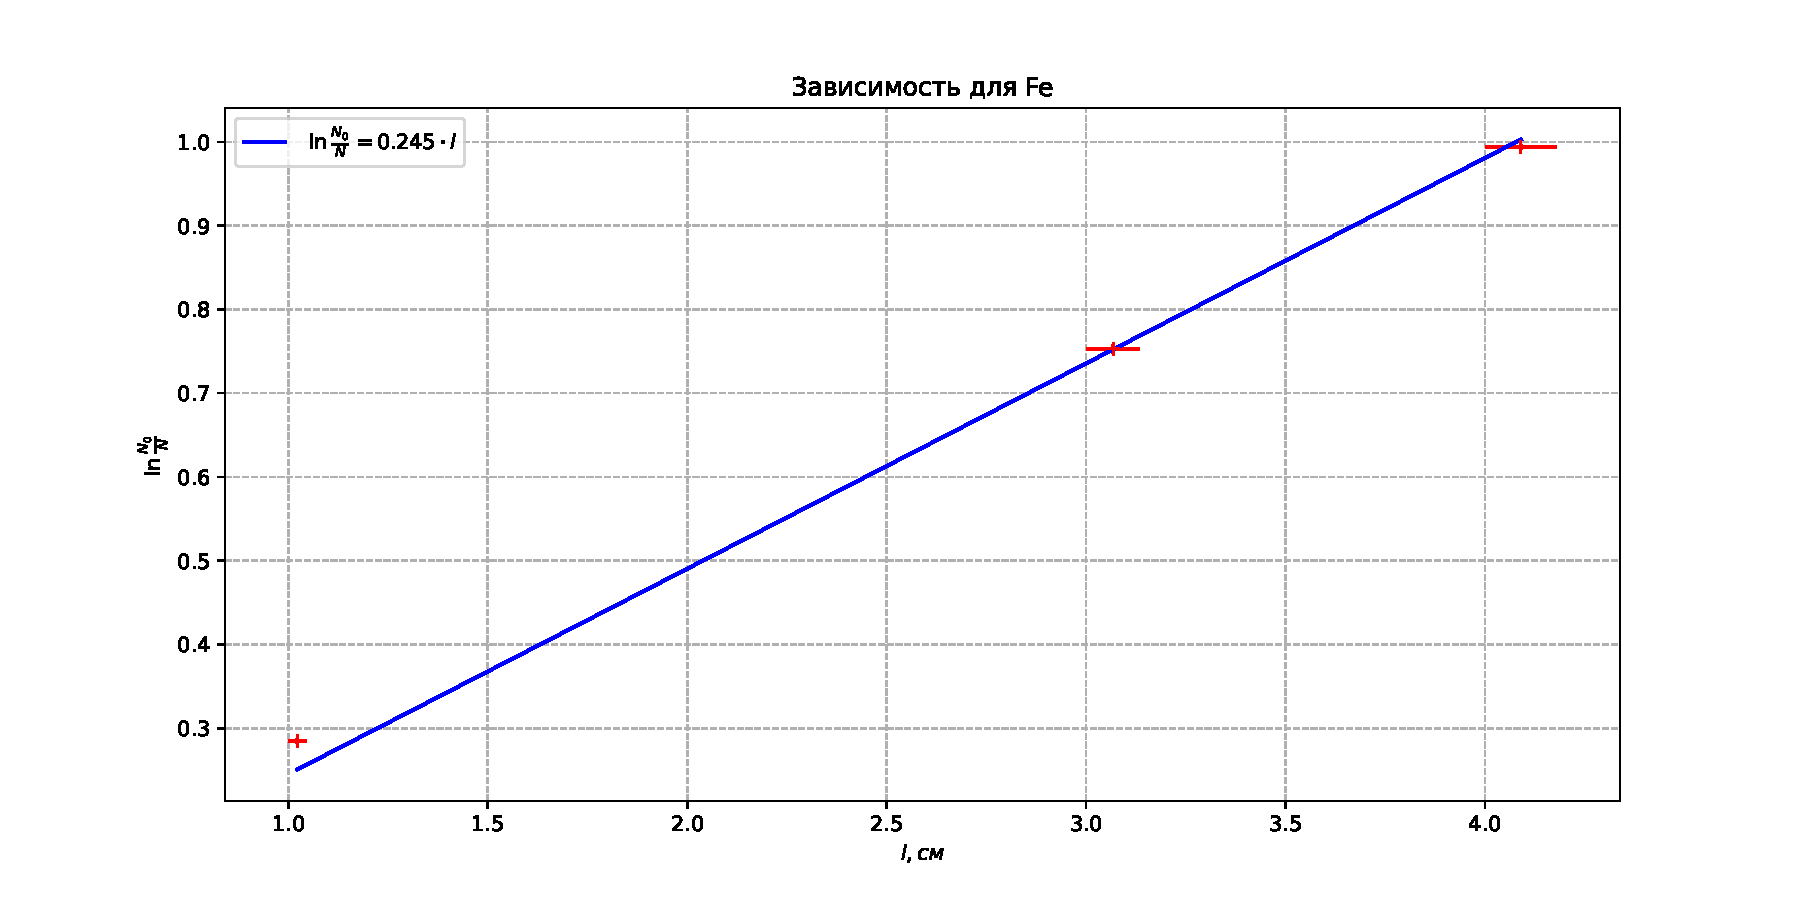
\includegraphics[width=1.0\textwidth]{pictures/graph_Fe.pdf}
	\caption{\textit{Зависимость $\ln \frac{N_0}{N}$ от $l$ для Fe}}
	\label{graph:2}
\end{figure}

\begin{figure}[!ht]
        \centering
	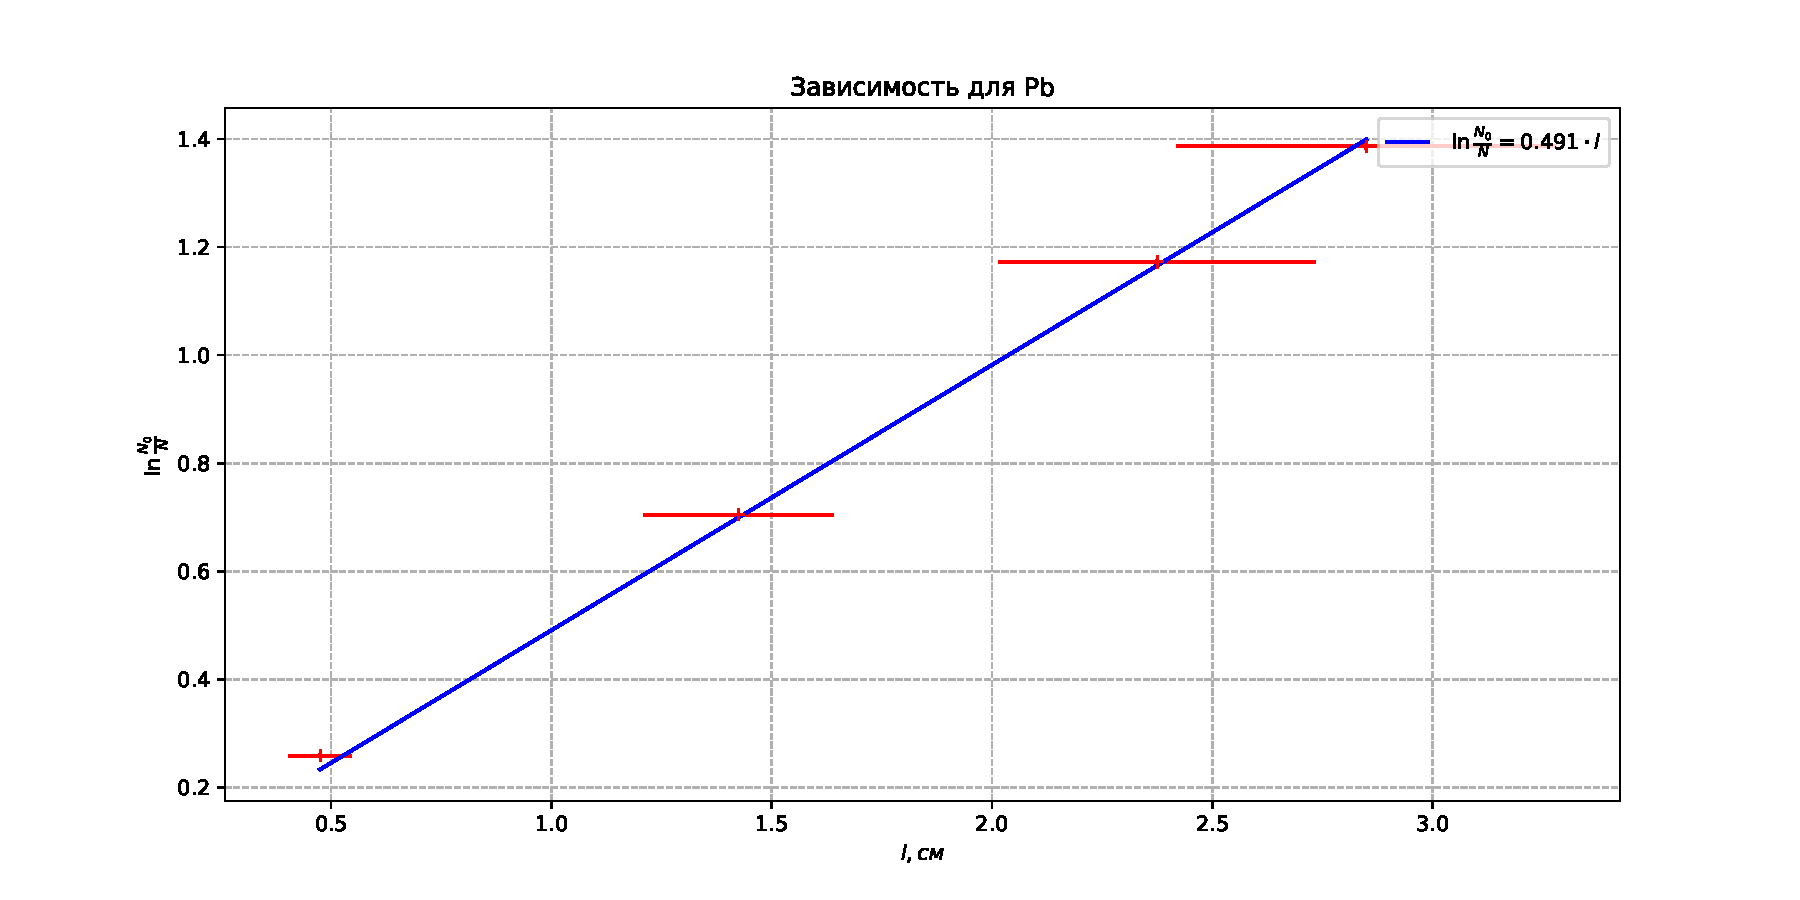
\includegraphics[width=1.0\textwidth]{pictures/graph_Pb.pdf}
	\caption{\textit{Зависимость $\ln \frac{N_0}{N}$ от $l$ для Pb}}
	\label{graph:3}
\end{figure}

\FloatBarrier


Коэффициенты ослабления найдем графически. 


\begin{equation*}
    \mu_\text{Al} = (0.182 \pm 0.006) \ \text{см}^{-1}
\end{equation*}
\begin{equation*}
    \mu_\text{Fe} = (0.245 &  \pm 0.005) \ \text{см}^{-1}
\end{equation*}
\begin{equation*}
    \mu_\text{Pb} = (0.491 \pm 0.004) \ \text{см}^{-1}
\end{equation*}

По линейным коэффициентам ослабления рассчитаем коэффициенты $\mu'$ из формул \eqref{eq:1} и \eqref{eq:2}.

\begin{equation*}
    \mu' = \frac{\mu}{\rho}
\end{equation*}



\begin{equation*}
    \mu'_\text{Al} = (0.067 \pm 0.002) \ \text{см}^{2}/\text{г}
\end{equation*}
\begin{equation*}
    \mu'_\text{Fe} = (0.0311 \pm 0.0006) \ \text{см}^{2}/\text{г}
\end{equation*}
\begin{equation*}
    \mu'_\text{Pb} = (0.0433 \pm 0.0004) \ \text{см}^{2}/\text{г}
\end{equation*}



\begin{enumerate}[resume]
    \item Используя найденные коэффициенты ослабления в свинце, железе и алюминии, по графику (рис. \ref{pic:mu_for_materials}) и таблице V.4 из Приложения V лабораторного практикума определим среднюю энергию $\gamma$-лучей, испускаемых источником. Представим их в таблице \ref{table:8}.
\end{enumerate}


\FloatBarrier
\begin{table}[!ht]
    \centering
    \begin{tabular}{|l|l|l|l|}
        \hline
        ~ & Al & Fe & Pb \\ \hline
        $\mu$, $\text{см}^{-1}$ & 0.182 & 0.245 & 0.491 \\ \hline
        $E_\gamma$, МэВ & 0.8 & 5.0 & 5.0 \\ \hline
    \end{tabular}
    \caption{Линейные коэффиценты ослабления и соответствующие им энергии для материалов}
    \label{table:8}
\end{table}
\FloatBarrier

\section{Выводы}

\begin{enumerate}
    \item В ходе работы были измерены линейные коэффициенты ослабления потока $\gamma$-лучей в свинце, железе и алюминии. Они представлены в таблице \ref{table:8}.
    \item По их величине была определена средняя энергия $\gamma$-квантов (см. таблицу \ref{table:8}).
\end{enumerate}


\end{document}
